\documentclass[12pt, a4paper, openany]{report}
\usepackage[left=3cm, top=3cm, bottom=3cm, right=4cm]{geometry}

\usepackage{mystyle}
\usepackage{csquotes}

\pagestyle{fancy}
\fancyhf{}
\lhead{kawa-i}
\chead{Bebarengan Sepur: Entlang der Schienen}
\rhead{\thepage}

\title{
    {Bebarengan Sepur - Entlang der Schienen}\\
    {\large{Ein Bildungsliverollenspiel}}\\
    {\bigskip}
    {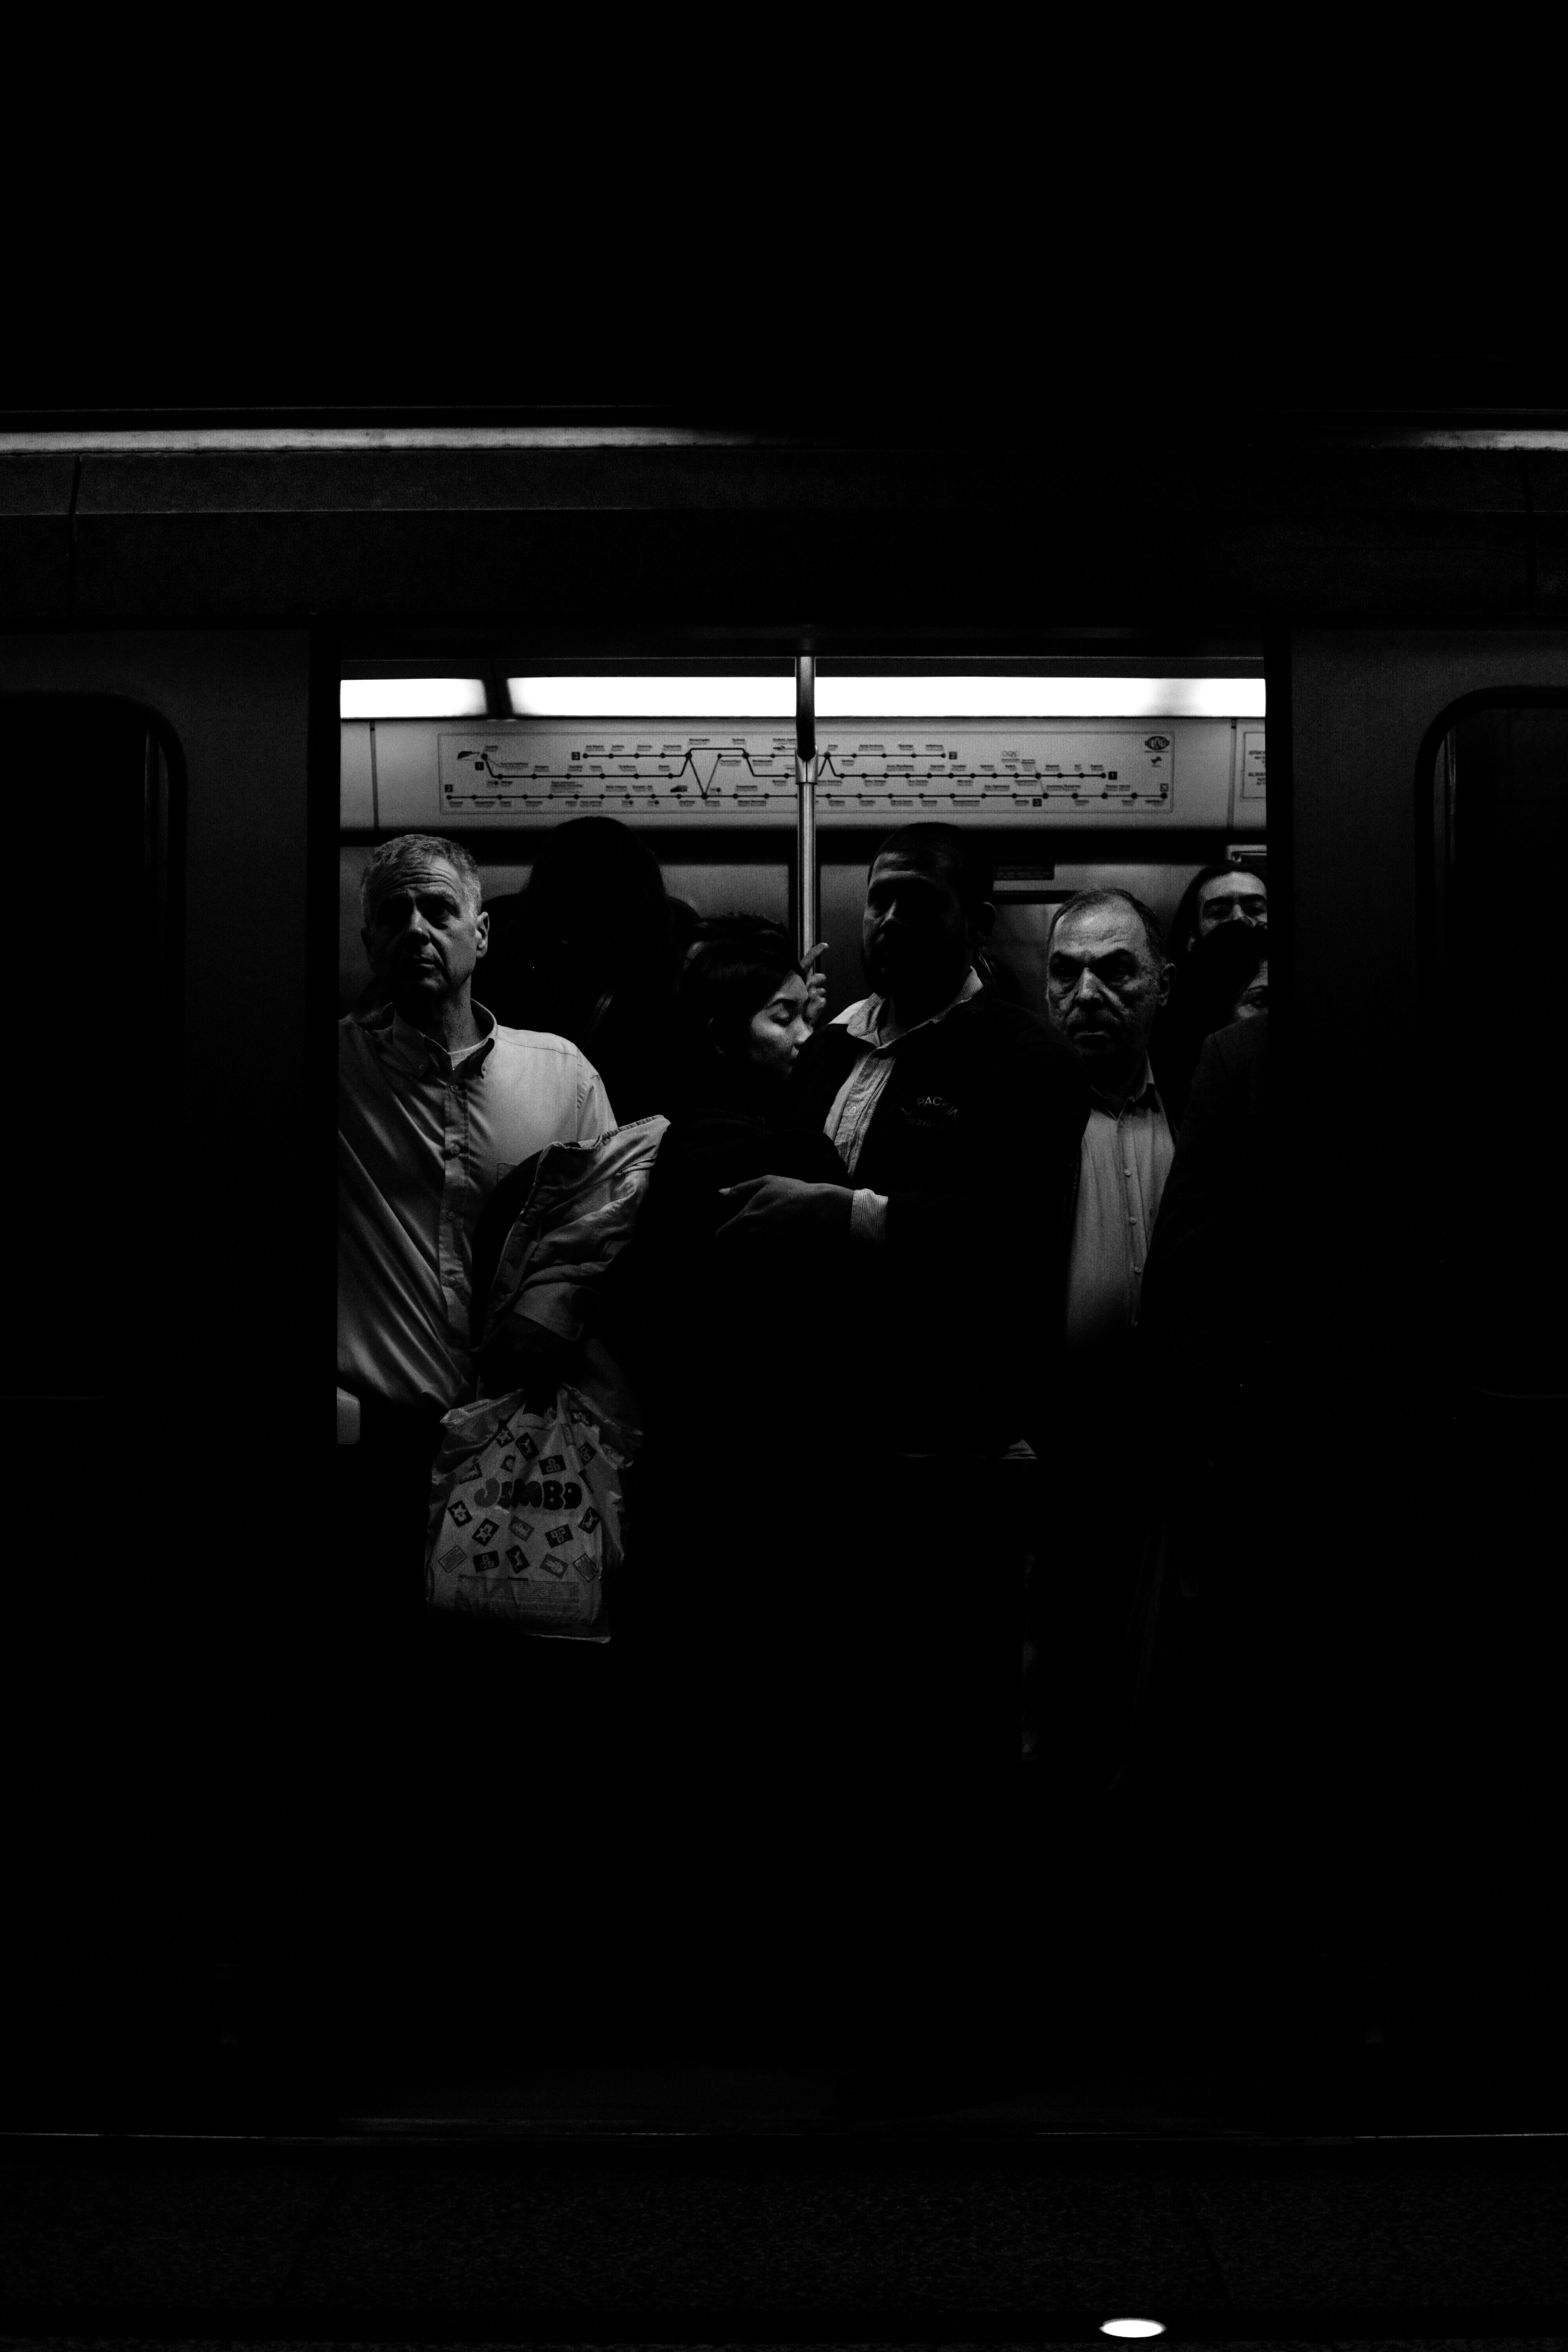
\includegraphics[scale=0.05]{title.jpg}}\\
}
\author{Orlando, fux, Equinox}
%\date{\today}

\begin{document}

\maketitle
\frontmatter
\tableofcontents
\mainmatter

\chapter{Einleitung}
\textit{Bebarengan Sepur - Entlang der Schienen} ist ein philosophisches Bildungsliverollenspiel, welches versucht, die Themen Freiheit, Autonomie und Befreiung in einen Kontext zu bringen mit den Problemen des 21. Jahrhunderts (Klimakatastrophen, Wirtschaftskrisen, Rechtsradikalismus etc.). 
Wir verbinden charakterbasiertes Liverollenspiel, angelehnt an \hyperref[nordic-larp]{Nordic Larp}, mit Kunst, Abstraktionen und surrealen Elementen. 
Die Erzählstruktur des Liverollenspiels greift Element genealogischer Kritik auf. 
Damit bilden \hyperref[kunst-abstraktion]{Kunst und Abstraktion}, sowie \hyperref[genealogische-kritik]{genealogische Kritik} die beiden Hauptmethoden zur Darstellung der Bildungsinhalte. 
Diese zwei Methoden haben wir durch die \hyperref[java-reihe]{Java-Reihe} hinweg entwickelt und weiterentwickelt und sollen in \textit{Bebarengan Sepur} das erste Mal zur vollen und spieltragenden Entfaltung kommen. 
So dienen sie hier nicht ausschließlich zu Darstellung der Bildungsinhalte, sondern bilden einen Hauptbestandteil bei der Konstruktion des Plots und der Spielgeschichte, sowie bei Erschaffung der Spielwelt.\\
Die Themen Freiheit, Autonomie und Befreiung greifen wir anhand der Perspektiven neuerer und älterer Kritischer Theorie (Adorno, Menke, Saar), sowie ihrer Vordenker*innen (Hegel, Marx, Nietzsche) auf. 
Theoretischer Hintergrund ist die Notwendigkeit der Befreiung aus der zweiten Natur, zum Einen als einzigem wirklichen Moment der Freiheit (Freiheit als Negation konkreter Unfreiheit), zum Anderen um fundierte Kritik an aktuellen Problemen zu formulieren.

\chapter{Game-Design}
\section{Spielsetting}
Das Spiel spielt in einer (dystopischen, aber auch \emph{noch} unklaren) Zukunft, in der was möglich ist noch ungewiss bleibt, jedenfalls für diese und jene Menschen. 
Menschen gehen ihren ganz gewöhnlichen Geschäften nach, aber hier und da gibt es Gerüchte, die Regierung würde Delinquenten statt sie ins Gefängnis zu bringen für Experimente nutzen. 
Wieder andere glauben an die Macht der Menschen, Träume kontrollieren zu können und zählen sich zu den sogenannten \qq{Träumenden}\todo[noline]{besserer Name}.\\
Wir befinden uns in, oder vor einer Zugfahrt auf die sich die Protagonisten unserer Geschichte vorbereiten.
Doch wo spielt sich diese Zugfahrt ab? 
Befinden unsere Protagonisten sich tatsächlich in dem Zug von St. Petersburg nach Moskau? 
Oder sind sie vielmehr Teilnehmer*innen an einem der Regierungsexperimente? 
Oder sind alle in einem gewaltigen Traum gefangen?\\

In so einer ungewissen Zeit und Welt stellen Kollektive und Gesellschaft für viele Menschen einen (seltsam) wichtigen Halt da. 
Doch da wir uns in der Zukunft und zugleich nicht in der befreiten Gesellschaft befinden, kann das nur bedeuten, dass wir im vorgeschrittenen kapitalistischen und liberalen Zeitalter uns befinden, wo die Menschen sich ihrer selbst und sich gegenseitig umso entfremdeter vorfinden, wie die Zeit die Schienen entlang rast.
Der Wunsch nach Kollektiven (Erfahrungen, Leidenschaften, Zusammensein) und die Macht der Vereinzelung, sind also sich umkreisende Pole unserer Geschichte.
So erzählt sich diese Geschichte in vier Akten, die diese Episoden von der Vereinzelung zur Kollektivierung verdeutlichen wollen: \emph{Der Raum}, \emph{Das Kollektiv}, \emph{Die Gesellschaft I}, \emph{Die Gesellschaft II}.

\section{Ein Liverollenspiel in vier Akten}
Das Liverollenspiel durchläuft vier Akte die jeweils mehrere Ebenen beinhalten: 1. die echte Realität (R) 2. Spielrealität (SR) 3. Metaebene (M) und 4. die philosophische Ebene (P). Innerhalb der Ebenen verläuft eine Entwicklung beispielsweise im Ausmaß und der Art der Interaktion der Spielenden, die alle Ebenen beeinflusst, da u.a. eine Entwicklung von Moral und somit einer zweiten Natur damit einher geht.
\subsection{Akt I - Der Raum}
\begin{itemize}
\item[R] Jede*r ist alleine in einem Raum in der Basa
\item[SR] ein Zugabteil 
\item[M] das Unterbewusste der Einzelnen
\item[P] Die Spieler*innen befinden sich auf dem subjektiven Standpunkt der Moral. 
\end{itemize}
Der Raum beinhaltet Gegenstände, die wesentlich für den bestimmten Charakter sind (z.B. ein Buch, Koffer?), evtl. gibt es eine Möglichkeit Musik abzuspielen, die inhaltlich etwas über die Vergangenheit der Person sagen könnte (\glqq hit me baby one more time\grqq{} oder altenglische Kirchenmusik von Henry Purcell) oder eine bestimmte Stimmung reproduziert.
 Es gibt 3 (oder mehr) mit Zahlenschlössern verschlossene Holzboxen, die in der Spielrealität Safes sein könnten, um Privatgegenstände auf dieser langen Reise im eigenen Zugabteil einschließen zu können.
Die Notizzettel mit den Zahlencodes wurden jedoch verloren.
Außerdem befindet sich ein Computer im Raum auf dem ein \hyperref[textadventure]{Textadventure} darauf wartet gespielt zu werden.\\
Link zum entsprechenden Akt im Textadventure: \hyperref[der-raum]{Der Raum}.

\subsection{Akt II - Das Kollektiv}
\begin{itemize}
\item[R] Die Tür des Raumes der Spieler*innen ist nun geöffnet, sie können den Gang betreten und treffen mit den mit den anderen Spieler*innen ihrer Etage zusammen.
Das Spiel kann nun auf der ganzen Etage stattfinden. 
Die Tür zur oberen, bzw. unteren Etage ist immernoch verschlossen.
\item[SR] Auf der Ebene der Spielrealität können sich die Spieler*innen nun frei in ihrem Waggon bewegen. 
Sie können die anderen Menschen im Zug treffen, mit ihnen reden und sich austauschen. 
In diesem Prozess finden sich die Menschen in Kollektive zusammen.
Die Spieler*innen werden am Ende des Zugabteils eine Tür mit der Aufschrift \glqq Tür deffekt\grqq{} vorfinden.
Diese Tür wird sich erst in Akt III öffnen.
\item[P] Auf der philosophischen Ebene treten die Spieler*innen aus dem bloß subjektiven Standpunkt ihrer persönlichen Moral heraus und betreten die objektive Welt der Sittlichkeit.
Das Gesetz der Objektivität, ihres Kollektives, tritt ihnen gegenüber.
In diesem Gesetzt können sie aber auch sich selbst erkennen und bilden an ihm ihr Wesen. 
Es bildet sich langsam die Sittlichkeit und die zweite Natur aus.
Auf dieser Eben kommt es allerdings noch nicht zu Konflikten und Widersprüchen, das Gefühl der Naturverkehrtheit wirkt authentisch, die Individuen geraten noch nicht mit ihm in Konflikt, das Gefühl der in Naturverkehrtheit wird erst im nächsten Akt entwickelt.
\end{itemize}
Link zum entsprechenden Akt im Textadventure: \hyperref[das-kollektiv]{Das Kollektiv}.

\subsection{Akt III - Die Gesellschaft Teil I}
\begin{itemize}
  \item[R] Es öffnen sich die Türen zwischen den zwei Ebenen/Gruppen. Diese vereinen sich nun und finden Ihre Rolle/Platz in dieser erweiterten \qq{Welt}
\item[SR] Die Züge/Krankenhausebenen vereinen sich und die Spieler treffen mit den Spielern/Kollektiven des jeweils anderen Teils aufeinander. 
Beim vereinen der Züge beschränkt ein Countdown das Vermischen der Gruppe auf eine endliche Zeit, vlt. 1 Stunde \hyperref[die-öffnung]{(Die Öffnung)}. 
Bei der zweiten Vereinigung ist die Öffnung permanent und die Spieler haben die Zeit ihre Rolle in den Kollektiven als auch die Rolle des Kollektivs in der vereinten Welt zu ergründen.
\item[M]
\item[P] Infragestellung, der 2. Natur durch die Begegnung mit anderen Kollektiven.
Durch diese Zusammenführung hervorgerufene Hinterfragung von Sittlichkeit, Rechtsverständnis und zweiter Natur im allgemeinen, stellt sich ein Bewusstsein oder Selbstbewusstsein der Naturverkertheit ein. 
\end{itemize}
Link zum entsprechenden Akt im Textadventure: \hyperref[die-gesellschaft]{Die Gesellschaft I}.

\subsection{Akt IV - Die Gesellschaft Teil II}
\begin{itemize} 
\item[R]siehe Akt 3
\item[SR] Alle befinden sich immer noch im Krankenhaus, jedoch vermuten inzwischen einige, oder wissen es (anscheinden) der Öffnung, dass es das nicht ist.
  Das Gefühl der Naturverkehrtheit, also das Hinterfragen der angenommenen so genannten zweiten Natur als Natur, hat eventuell zur Auflösung der vorhandenen Kollektive geführt. 
    Auch möglich ist jedoch eine Verhärtung der Fronten, also eine noch verstärkte Identifikation über die eigene Gruppe bis hin zur Totalität, weil die eigenen Vorstellungen nur noch haltbar sind, wenn sich vollkommen abgegrenzt wird von denen die anders denken. 
    Zur Verschärfung des Konflikts zwischen den Kollektiven oder dem Beenden der Situation (R: des Spiels) durch Zusammenführung in eine große Gesellschaft braucht es konkrete Ziele in den Charakteren oder/und den Kollektiven zB.: 
    die Experimente in eine bestimmte Richtung zu leiten/manipulieren durch die Eingeweihten (oder jene, die Glauben es zu sein), ein krankenhausinternes Ereignis, wie Ressourcenknappheit aufgrund einer Klimakatastrophe (Sturmflut) und somit der \qq{gesamtgesellschaftlichen} Aufgabe Medizin u.ä. aufzuteilen. 
    Auch abstrakte Bestrebungen und Phobien der Kollektive (Abneigung der Farbe Gelb gegenüber) kommen spätestens jetzt zur Kollision. 
\item[M] 
\item[P]Ein oder mehrere totalitäre Gruppen sind entstanden oder Aufhebung aller Werte und Friede-Freude-Feierkuchen-Welt auf einer Wiese
\end{itemize}

Link zum entsprechenden Akt im Textadventure: \hyperref[die-gesellschaft2]{Die Gesellschaft II}.

\section{Die Kollektive}
Im Laufe des Spiels bilden die Spieler*innen anhand ihrer Charakterbeschreibungen, also vorherigen Zuordnung, drei Kollektive. 
Innerhalb dieser Kollektive bildet sich ein jeweiliger Kollektiv-Konsens (wie genau das passiert, ist noch unklar), man könnte auch davon sprechen, dass sich in jedem Kollektiv eine \hyperref[zweite-natur]{\glqq zweite Natur\grqq{}} bildet. 
Das Eingehen jedes einzelnen Charakters in das Kollektiv, soll sich auch im Charakter widerspiegeln (beispielsweise in seinem Raum) 
Die Identität des Kollektivs speist sich aus der der Individuen, gleichzeitig verändert sie aber auch die Individuen selbst. 
Hier wird versucht ein Aspekt Hegels-Philosophie zu verdeutlichen. 
Bezug genommen wird speziell auf drei Passagen der Hegelschen Rechtsphilosophie: \\

\begin{itemize}
    \item[] \qq{Das objektiv Sittliche, das an die Stelle des Abstrakten Guten tritt, ist durch die Subjektivität [...] konkrete Substanz.}\footfullcite[][§ 124, S. 161]{hegel_grundlinien_2017} \\
    \item[] \qq{Andererseits sind sie [die Gesetze des des objektiv Sittlichen] dem Subjekte nicht ein Fremdes, sondern es gibt das Zeugnis des Geistes von ihnen als von seinem eigenen Wesen.}\footcite[][§ 147, S. 162]{hegel_grundlinien_2017} \\
    \item[] \qq{Aber in der einfachen \emph{Identität} mit der Wirklichkeit der Individuen erscheint das Sittliche, als die allgemeine Handlungsweise derselben - als \emph{Sitte}, - die \emph{Gewohnheit} desselben als eine \emph{zweite Natur}}\footcite[][§151, S. 166]{hegel_grundlinien_2017}
\end{itemize}

Ideen zu den Kollektiven:
\begin{itemize}
\item Reproduktionsarbeit (z.B. kochen, Zug antreiben, Heizraum abkühlen), also Aufgaben, die Verwaltung bedürfen.
\item Keine politischen Konzepte für die Kollektive, diese entwickeln sich aus den Charakteren 
\item (Skurriles) Sammelsurium an Regeln, der Gruppe (z.B. alles Grüne abdecken)
\end{itemize}

Die drei Kollektive unterscheiden sich auf verschiedenen Ebenen. 
Dazu gehören vor allem 1. eine andere Wahrnehmung der Realität (Zug/ Krankenhaus, Experiment, Traum) und 2. ein Ziel, dass sie vereint.

\subsection{Kollektiv - Zug/ Krankenhaus}
Dieses Kollektiv hat keinen Hintergedanken zu (seiner) Wirklichkeit und glaubt schlicht in einem Zug und später einem Krankenhaus zu sein. 
Dieses Kollektiv ist vollständig auf Etage zwei platziert. 

\subsection{Kollektiv - Schlaf/ Traum}
Dieses Kollektiv nimmt an, dass sie in einem Traum gefangen sind der bestimmte Erfahrungen vorgaukeln will (aus welchen Gründen?).
Es müssen nicht alle Charaktere dieses Kollektives davon wissen, aber es sollte irgendwo in der Charakterbeschreibung zumindest einen Hinweis darauf geben.
Diese Gruppe könnte das Ziel haben/ entwickeln, den Zug zu Kapern (vielleicht mit dem Hintergedanke dadurch den Traum steuern zu können).
Dieser Hintergedanke könnte sich so weiterentwickeln, dass sie versuchen den Zug zu kapern um einen ewigen Traum einzuleiten, in dem es Frieden und Wohlstand und Erfüllung sämtlicher Wünsche und Begierden gibt? (Naruto: Madara)
Dieses Kollektiv befinden sich vollständige auf Etage eins.

\subsection{Kollektiv - Experimente}
Dieses Kollektiv glaubt, dass sie in dem Zug sind, aber, dass die ganze Zugfahrt/der Krankenhausaufenthalt ein Experiment ist. 
In diesem Kollektiv befinden sich außerdem Menschen, die glauben die Durchführer*innen eines dieser Experimente zu sein.
Dieses Kollektiv ist teilweise auf Etage eins, teilweise auf Etage zwei.\\

Es ist nochmals hervorzuheben, dass alles was passiert in jeder Geschichte eine konsistente Erzählstruktur braucht. 
Also zum Beispiel der Cut, oder die Geschichte, die nach dem Cut den Charakter ins Krankenhaus führt, muss \emph{aus jeder} Kollektivperspektive erklärbar sein.
Damit sich nicht in unseren Erzählstrukturen ein (ungewollter) Hinweis darauf besteht, dass eine der Kollektivperspektiven die Wirkliche\footnote{Natürliche sind alle Perspektiven, wie \hyperref[realitaeten]{im Folgenden} erklärt im eigentlichen Sinne \emph{wirk}ich} ist.
Wenn der Cut z.B. wie in Issue 17 vorgeschlagen wurde, dadurch zustande kommt, dass das Schlaf-Kollektiv\todo[noline]{Wir brauchen gute Namen für die Kollektive} den Zug kapern möchte, dann ließe sich der Cut konsistent aus allen drei Perspektiven gut erklären:
\begin{itemize}
    \item[Kollektiv 1:] Der Zug ist Infolge der Aufruhr (tatsächlich) entgleist.
    \item[Kollektiv 2:] Die Aufregung in den Charakteren haben sie dazu
      veranlasst aus dem Traum aufzuwachen und in einen neuen Traum zu wecheln.
    \item[Kollektiv 3:] Das Experiment wurde auf Grund der Aufruhr abgebrochen.
\end{itemize}

\section{Die Realitäten}\label{realitaeten}
Die Frage nach der Realitäten ist auf mehrfache Weise interessant. 
Zum einen die Frage, wie sich die einzelnen (angenommenen) Realitäten der Kollektive logisch erklären. 
Diese müssen, denke ich, alle eine gewisse Konsistenz aufweisen.
Außerdem ist die Frage, was \emph{für uns} die Realität ist, und ob wir eine solche brauchen.\\

Eine Idee dazu: die Realität ist, dass es verschiedene Realitäten gibt, dass die Wirklichkeit nichts außer \emph{Schein} ist.
Das ist der gemeinsame Nenner, der sich in allen Realitäten zeigt.\\
Das soll kurz erklärt sein: 
im Gegensatz zum reinen/ radikalen Dekonstruktivismus, der davon ausgeht, dass es kein eigentlich Seiendes gibt, zumindest keines, dass nicht konstruiert ist, sondern nur die von mir konstruierte Wirklichkeit (kein \emph{An-Sich}, sondern nur \emph{Für-Uns})%
\footnote{Hier gibt es Unterschiede, ob zumindest die Erscheinung für Menschen aus bestimmten Gruppen die gleiche ist, oder, ob sie wirklich rein individuell ist.}%
, nimmt eine materialistisch-dialektische Philosophie stets an, \emph{das etwas} erscheint.
Also es gibt zumindest ein Sein (etwas das Existiert), was \emph{als etwas} erscheint.
Beispielsweise: 
ein Handy erscheint uns als ein sinnvoller Gegenstand, mit dem wir jederzeit mit allen Menschen in Kontakt treten können.
Einem Jakobiner während der Französischen Revolution, wäre es bestenfalls als Waffe zum Erschlagen von Aristokraten erschienen.
Aber es gibt zumindest diesen Gegenstand, der als Handy, oder als Waffe erscheint.
Nun würde zwar auch ein (materialistischer) Dialektiker, behaupten, dass der Schein die \emph{Wirk}lichkeit ist, da sie das ist, was auf uns wirkt, uns beeinflusst, worauf wir reagieren, aber es muss eben immer auch das geben, \emph{was} erscheint. 
Und zumindest das ist das \emph{nicht-konstruierte}, welches wir aber nie erreichen können, von dem wir nur (durch z.B. Kunst) eine Ahnung erhaschen können.
Adorno nennt dies das \qq{Nichtidentische}.
Nun meine ich, dass es hier ebenso nicht darum gehen kann zu sagen: 
\qq{schaut her, es gibt gar nicht so was wie echtes Sein, alles ist nur Schein, jeder kann in seiner Traumwelt leben, wie er will}, sondern, dass es zumindest das Eine geben muss, \emph{was} erscheint. 
Mein Vorschlag ist nun folgender: wenn nur etwas wie Kunst, oder Erfahrung, o.ä. uns das Hinter-dem-Schein-Liegende zeigen kann, und dass was Kunst uns zeigt, immer notwendig etwas Abstraktes bleibt (abstrakt in dem Sinne, dass wir es nie (mit Begriffen) ganz greifen können, dass es die Kunst gewissermaßen auszeichnet, \emph{flüchtig} zu bleiben, wir können sie nie ganz in der Hand halten, dingfest machen), dann wäre es doch interessant, wenn dasjenige, was die Kunst uns nur in dieser Flüchtigkeit, in dieser Abstraktheit zeigen kann, selbst etwas abstraktes ist: also kein eigentliches Sein, sondern nur, gewissermaßen die \emph{Idee}, dass es an der Oberfläche eben immer nur Schein gibt. 
Das würde dann weiter bedeuten, dass es in den abstrakten Momenten des Spiels eben (auch) darum geht, diesen Wirklichkeitscharakter des Scheins, zu zeigen: 
\qq{Schein ist das Wirkende und Lebende selber}\footfullcite[][417]{nietzsche_morgenrote_1999}. 
Aber genauso, dass er nur Schein ist und dass wir daher den Schein der Notwendigkeit (der ja da ist, solange wir nicht wissen, dass es Schein ist) zu durchstoßen.\footcite[Vgl.][41]{menke_autonomie_2018}
Dass wir letztendlich einen Schein erschaffen müssen, der \qq{so weit in seiner Selbstverspottung geht, mich fühlen zu lassen, dass hier Schein und Irrlich und Geistertanz und nichts Mehr ist}\footcite[][417]{nietzsche_morgenrote_1999}.

\subsection{Das Experiment}
Was sind die Experimente? wieso werden sie durchgeführt? Wie werden sie durchgeführt?

\subsection{Die Träume}
Wieso? Wie? Unter welchen Bedingungen?

\subsection{Die Realität}
Was gibt es für das 1. Kollektiv vielleicht als Background Fakts zu der Zugfahrt/ dem Krankenhaus?



\section{Die Öffnung/ Der Cut} \label{die-öffnung}
\todo{Was bedeutet das auf der Spielrealitätsebene, was wird den Spieler*innen vermittelt}    
Erreichen die Spieler*inner innerhalb des zweiten Aktes des ersten Teils einen bestimmten Punkt, öffnen sich erstmals die beiden Abteile/ Etagen. 
Es beginnt ein Countdown in Sekunden, begleitet von \textit{koyaanisqatsi} von Philipp Glas. 
Während dieser Phase können sich erstmals alle Charaktere begegnen. 
Am Ende des Countdowns wird ein \hyperref[cut]{Cut} initiert, das Spiel geht kurz OT und alle Spieler*innen werden wieder auf ihr Zimmer geschickt. 
Evtl. gehen alle Spieler*innen schlafen.  

\section{Erfahrungen}
Entscheidend ist auch die Frage, welche Erfahrungen die Teilnehmer*innen Konkret machen sollen.
Parallel zu den Akten und der Entwicklung, sollen auch bei den Teilnehmer*innen Erfahrung erzeugt werden, die sich in diese Ordnung einsortieren lassen:
\begin{itemize}
\item Selbstkonflikt, wer bin ich? (Akt I - Der Raum)
\item Identifizierung (Akt II - Das Kollektiv)
\item Scheitern (Akt III - Die Gesellschaft Teil I)
\item Reflexion: Versönung/ Katastrophe (Akt IV - Die Gesellschaft Teil II)
Im Folgenden soll auf die Erfahrungen und die Verbindungen zu den Akten näher eingegangen werden.
\end{itemize}

\chapter{Part One - Der Zug}
\section{Spielsetting}
\section{Spielrealität}
\section{Die Gruppen}
\subsection{Gruppe 1}
\subsection{Gruppe 2}
\subsection{Gruppe 3}
\section{Akt I}
\section{Akt II}

\chapter{Part Two - Krankenhaus}
\section{Spielsetting}
\section{Spielrealität}
\section{Die Gruppen}
\subsection{Gruppe 1}
\subsection{Gruppe 2}
\subsection{Gruppe 3}
\section{Akt I}
\section{Akt II}
\section{Akt III}
\section{Akt IV}



\chapter{Traum Raum}
Neben dem Hauptgeschehen, sollen in einzelnen Bereichen Nebenstränge aufgemacht, oder zusätzliche Erfahrungen gemacht werden können. 
Neben dem \hyperref[textadventure]{Textadventure} ist der sog. \glqq Traum Raum\grqq{} eines dieser Orte.
Hier sollen den Spieler*innen verschiedene Träume vorgeführt werden. 
Bzw. es wird ihnen ein Traum gezeigt, auf den sie selbst Einfluss nehmen können (luzid dreaming?).
Dies soll mit einer einfachen Texteingabe geschehen.
Den Teilnehmer*innen werden Fragen gestellt und die \glqq Künstliche Intelligenz\grqq{} reagiert auf bestimmte Stichwörter und führt je nach Wort den Traum auf andere Art und Weise fort.
Zugleich werden die einzelnen Traumsequenzen bestimmten Kategorien zugeordnet, die sich mit den \hyperref[minds]{Minds} verknüpfen lassen.
Dadurch sollen die Entscheidungen der einzelnen Spieler*innen Einfluss auf das Textadventure ausüben können (indem sich die Minds verändern, verändert sich damit auch der Text im Textadventure).
Wenn es gut gelingt vom Textadventure eine Rückkopplung auf das eigentliche Spiel zu erzeugen, kann damit eine generelle Wechselwirkung zwischen Spiel und Textadventure stattfinden.
Der Traum selbst wird in Form von Videos dargestellt die abgespielt werden.\\

Weitere (Wunsch-) Vorstellungen:
\begin{itemize}
\item Statt Texteingabe Spracherkennung und die Fragen werden vorgelesen.
    Nach kurzer Recherche konnte ich zum Beispiel diese Bibliothek finden: \href{https://github.com/Uberi/speech_recognition}{Uberi}. \todo{Alex, wie siehst du da die Möglichkeiten?}
\item Wie werden die Videos gezeigt? 
    Leicht zu realisieren wäre zum Beispiel Leinwand + Beamer, wobei das etwas langweilig ist. 
    Hammer wäre natürlich die Videos über eine VR-Brille zu zeigen, was in Kombination mit dem gesprochenen Text und der Voice recognition ein \glqq traumhaftes\grqq{} Bild abgeben würde.
    Etwas realistischer sind vielleicht mehrere Computerbildschirme, die die Videos (evtl. leicht versetzt) abspielen? 
\end{itemize}

\chapter{Textadventure} \label{textadventure} 
Das Textadventure \textit{Der Zug} spielt eine zentrale Rolle innerhalb des Liverollenspiels und ist eine wichtige Ergänzung in der die Konzepte des Spiels auf einer weiteren Ebene verdeutlicht werden sollen. 
\textit{Der Zug} zielt sowohl darauf ab, verschiedene Medien in Liverollenspiel zu integrieren, als auch verschiedene Medien zu Vermittlung von Bildungsinhalten nutzbar zu machen, bzw. die Benutzbarkeit verschiedener Medien zur Vermittlung sicht- und denkbar zu machen.\\
Stickpunkte (Wozu ist das Textadventure da):
\begin{itemize}
\item Darstellung des Unterbewusstseins (Traum)
\item Beeinflussung der Spieler*innen durch das textadventure
\item Einleitung in das Spiel (ersten Akt)
\item (Geheime) Begegnung mit anderen Spieler*innen (weitere Akte)
\item Zusätzliche Informationen für die Spieler*innen
\item Entwicklung des Bewusstseins (Aspekte dialektischer Philosophie einbinden)
\end{itemize}
In dem Abschnitt \hyperref[txtad-anlehnung]{5. 7} werden Teile dieser Aspekte nochmals aufgegriffen.

Negative Aspekte:
\begin{itemize}
\item Kampfsystem?
\item Nimmt es in Zukunft zu viel Raum ein? 
\end{itemize}
Die Negativen Aspekte wurde diskutiert.
Erstmal wurde sich darauf geeinigt, dass das Spiel nach dem ersten Akt nicht mehr überaus viel Einfluss hat und Raum einnimmt, so dass es hauptsächlich während des ersten Akts, in welchem viele Charaktere noch kaum Speiler*innen-Kontakt haben present ist, bzw. präsens fordert.
Uneinig sind wir uns noch über den Abschnitt im Krankenhaus.\\

Während das Liverollenspiel selbst äußerlich in zwei Teile aufgeteilt ist (\textit{Der Zug} und \textit{Die Anstalt}), verdeutlicht das eingegliederte Textadventure die innere Aufteilung in drei Akte: 
\begin{itemize}
\item[I] Der Raum
\item[II] Das Kollektiv 
\item[III] Die Gesellschaft - Teil I
\item[IV] Die Gesellschaft - Teil II
\end{itemize}
Während in dem Liverollenspiel selbst diese drei Akte sich nacheinander entfalten, greift das Spiel auf jeder Ebene 1. in abstrakter Form/ auf einer Metaebene auf die nächste Ebene zu und öffnet 2. währende der Öffnung schon hin zum nächsten Akt. \\
Im Gegensatz zu \glqq gewöhnlichen\grqq{} Textadventure, ist es eher angelehnt an ein Openworld Rollenspiel, in dem sich der Charakter zu jeder Zeit frei bewegen kann.
Das heißt, er befindet sich in einem Raum und kann sich mittels verschiedene \textit{Befehle} z.B. Gegenstände oder Personen in seinem Raum anzeigen lassen, er kann mit diesen in Interaktion treten/ sie ins Inventar aufnehmen, er kann sich die benachbarten Räume anzeigen lassen und diese Wechseln. 
Beim Betreten eines Raumes, wird eine grobe Beschreibung des Raumes, dessen, was der Charakter sieht, ausgegeben. 
Es wird also versucht die Welt eines gewöhnlichen (PC-) Rollenspiels mittels literarischer Beschreibung zu visualisieren. \\
Der Aktwechsel innerhalb des Textadventures geschieht parallel zu dem realen Aktwechseln. \todo{Bilder einf\"ugen vom Spiel}

\section{Der Raum} \label{der-raum}
Wie die Charaktere zu Beginn in einzelnen (oder Gruppen-) Räumen sind, befindet sich der Spieler/ die Spielerin zu Beginn alleine in einem Zugabteil. 
Alleine bis auf einen Begleiter, \textit{Parsen}.
Der Charakter in seinem Abteil, kann dieses nicht verlassen. 
Der Ausgang \glqq Tür auf den Gang\grqq{} wird zwar angezeigt, aber bei dem Versuchen diesen auszuwählen, tritt der Spieler wider Erwarten nicht auf den Gang des Zuges, sondern befindet sich in dem Foyer eines Krankenhauses. 
In der Welt in der der Spieler sich nun befindet, ist eine Zombieapokalypse ausgebrochen. \todo{Es wäre zu überlegen, ob das das beste Setting ist :D}
Egal wie der Spieler sich entscheidet, dieses kleine \hyperref[zombieapokalypse]{Mini-Spiel} endet immer damit, dass der Spieler aus dem Krankenhaus flüchtet und wieder in seinem Abteil auftaucht.
Das geschieht so lange, bis der Spieler auch im eigentlichen Rollenspiel seine Tür geöffnet hat.
Ab dann betritt er bei Wählen dieses Ausgangs tatsächlich den Gang des Zuges.\\
Wie also im Liverollenspiel selbst, bleibt der \glqq natürtliche\grqq{} Übergang in den zweiten Akt an bestimmte Ereignisse in dem \glqq realen\grqq{} ersten Akt verknüpft. 
Allerdings eröffnet der Dialog mit dem geheimnisvollen Begleiter, Parsen, eine Möglichkeit vorab in Szenen des zweiten Akts einzutauchen: 
\begin{itemize}
\item[] Neben normalen Dialogoptionen, die bei jeden Charakter anders sind und die Möglichkeit bieten in die Hintergrundgeschichte des Charakters einzutauchen und neue Aspekte des Charakters kennenzulernen (also wiederrum Darstellung des Innenlebens des Charakters, wie im realen ersten Akt die Bilder, die Musik, etc. des Raumes), kann jeden Charakter im Dialog mit Parsen von einem Traum erzählen. 
Dieser Traum entwirft ein weiteres kleines (Rollen-) Spiel, welches durch Fragen von Parsen konstruiert wird, á la \textit{und was ist dann passiert? ...}. 
Innerhalb dieses Fragen-Antwort-Spiels, kann der jeweilige Charakter alle Charaktere seines (späteren) Kollektives treffen.
Sofern diese gerade auch im Spiel sind, sogar real mit Ihnen schreiben. (\textit{\frqq hast du mit ihm gesprochen?\flqq{} \frqq Ja\flqq.} $\rightarrow$ Dann beginnt der Dialog mit diesem Spieler).
Insofern ist das Textadventure teilweise ein mprpg (Multiplayer Roleplaying-Game).
\end{itemize}

\section{Das Kollektiv} \label{das-kollektiv}
Im zweiten Akt steht dem Spieler der Zugang zu dem Gang des Zuges frei. 
Er kann nun also real mit allen Charakteren aus dem zuvor erzählten Traum kommunizieren und ihnen auch begegenen, außerdem aber mit allen weiteren Charakteren, also allen Charakteren, die nicht Teil seines Kollektives sind. \\
An dieser Stelle fehlt noch ein Konzept, um die Trennung zwischen Kollektiv und Nicht-Kollektiv-Mitglieder darzustellen.
Möglicher Konzeptvorschlag:
\begin{itemize}
\item[] Alle Mitgleider des Kollektives befinden sich in einem bestimmten Abschnitt des Zuges (z.B. im Bordbistro), während alle übrigen Charaktere sich in den verschiedenen Zugabteilen befinden.
\end{itemize}

In diesem Akt kann durch etwas, wie ein Bug auf den nächsten Akt zugegriffen werden: 
durch einen Raum betritt man plötzlich eine scheinbar magische Welt:
man verlässt den Zug und ist in einem anderen Setting (saftig grüne Wiesen, Wälder, Blumen, blauer Himmel etc.).
Hier tritt erstmals eine harmonische Gesellschaft auf. 
Allerdings besteht diese Gesellschaft zunächst nur aus den Mitgleidern des Kollektives und zeigt noch die Fehlerhaftigkeit der Gesellschaft: es gibt noch ausgeschlossene, es gibt noch totalitäre Strukturen: die Gesellschaft \textit{wirkt} wie eine Gesellschaft, ist aber noch in der Form eines Kollektives. 

\section{Die Gesellschaft - Teil I} \label{die-gesellschaft}
Die Gesellschaft findet nun nur noch in dieser traumhaften Welt der saftigen Wiesen, der Blumen und des perfekt blauen Himmels statt. 
Die Gesellschaft ist vereint und scheinbar perfekt. 
In dem Liverollenspiel ist der dritte Akt gerade der Akt, im dem die Konflikte zwischen den Kollektiven und innerhalb der Kollektive ausgetragen wird. 
Die \textit{Struktur} in der eine Versönung stattfinden kann ist aber schon gegeben. 
Nur innerhalb dieser Struktur, in der die Menschen zusammenkommen und über sich (und zweite Natur) reflektieren, kann eine Befreiung, wirkliche Autonomie etc. erreicht werden.
Das Textadventure greift also auch hier wieder eine Ebene voraus: die Struktur ist schon gegeben, aber auch der Inhalt scheint vorzuliegen: alle Menschen sind in dieser schönen Welt vereint und Widersprüche sind nur versteckt zu finden.
Der noch vorhandene Widerspruch ist dargestellt durch die Möglichkeit der Rückkehr in den Zug, aber auch in einzelnen Gegenständen.
So besteht zum Beispiel die Welt aus mehreren Bereichen: Lichten, Wald, See. 
Der See wird zu dem abschießenden Spiegel, in dem nochmals alles Reflektiert wird.
In einem großen Dialog, können hier nochmals alle Entwicklungsschritte und Widersprüche und Konflikte durchgemacht werden.

\section{Die Gesellschaft - Teil II} \label{die-gesellschaft2}
Der vierte Akt im Liverollenspiel stellt die Phase der Entscheidung dar. 
Die Spieler*innen und Kollektive haben ihre Konflikte ausgetragen und es fragt sich, ob eine neue Geslelchaft auf höherer Ebene erreicht werden kann, oder nicht; dann würde die Barbarei folgen.
Hier sind zwei Möglichkeiten eines Ausgangs beschrieben und die mögliche Darstellung im Textadventure: falls die Spieler*innen innerhalb des eigentlichen Liverollenspiels...
\begin{itemize}
\item[1.] ... in eine harmonische Gesellschaft übergehen, also die Widersprüche auflösen können, wird im Textadventure beschrieben, wie der Zug abfährt, während alle Spieler*innen auf den saftigen Wiesen und Feldern stehen. 
(Falls man es noch etwas dramatischer haben mag, könnten alle Menschen nach Abfahrt des Zuges auf den See zu gehen und mit ihm eins werden.)
\item[2.] ... den Zerfall der Gemeinschaft herbeiführen, versinkt alles im Chaos: die harmonische Welt zerfällt, die Spieler*innen befinden sich plötzlich wieder in ihrem Zugabteil, der Zug fährt los und entgleist. 
(Dramatische Alternative: unter den Spieler*innen bricht Panik aus, sie rennen davon und überstürzt in den See.
Sie fallen in den See, verlieren kurz ihr Bewusstsein und wachen in ihrem Zugabteil wieder auf der Zug fährt los und a) das Spiel geht von vorne los, b) der Zug entgleist.)
\end{itemize}

\section{Mini-Spiel: Zombieapokalypse} \label{zombieapokalypse}
Idee des Spiels:
\begin{itemize}
\item Verbindung zur realen Welt (Kamp gegen das System)
\item Kampf gegen die sieben Todsünden (dann auch Entrückung am Tage des Jüngsten Gerichts)
\end{itemize}
Zumindest in diesem Teil des Textadventures wird es ein Kampsystemgeben. \todo{Frage wäre, ob es ein Kampfsystem vielleicht auch ansonsten gibt}
Der Spieler befindet sich in dem Foyer eines Krnakenhauses und entdeckt langsam, dass die meisten Menschen dort Zombies sind, die gerade dabei sind die Ärzte zu überwältigen. 
Evtl. könnte der Spieler die Option haben sich den Ärzten oder dne Zombies anzuschließen.
Egal welche Option er wählt, dieses kleine Mini-Spiel wird immer damit enden, dass der Spieler wieder in seinem Abteil endet, nachdem er versucht aus dem Krankenhaus zu flüchten.

\section{Minds}\label{minds}
Ein weiteres Konzept des Textadventures, welches hier beschreiben und ausgearbeitet werden soll, ist der der \glqq Minds\grqq{}.
Dieses Konzept, welches uns in dem RPG \glqq Disco Elisium\grqq{} begegnete, lässt das Geschriebene, also die Welt des Spielers, durch verschiedene Charaktäre, hier \textit{Minds}, erzählen.
Während Disco Elisium Charactere, wie \textit{Logik, Perzeption, Drama, Enzyclopädisches Wissen etc.} benutzt, die sich leicht auf das Geschriebene Abbilden: Logik erklärt einen komplexen Zusammenhang, Enzyclopädisches Wissen beschreibt dem Spieler die Vogelart, die er sieht, etc., wollen wir versuchen die Entwicklung des Geistes in Hegels Phänemenologie darzustellen, indem die Minds die entsprechenden Stufen des Geistes darstellen: Bewusstsein, Selbstbewusstsein, Geist, Religion, Das absolute Wissen.
Dabei sollen diese Stufen sich auf der einen Seite parallel zum Spiel und zu den Akten entfallten und andererseits skillbare Attribute des Spielers sein:
jenachdem, welche Eigenschaften der oder die Spieler*in trainiert, soll die Beschreibung der Welt für den Spieler anders aussehen. 
Diese beiden Aspekte zusammenzubringen, ohne völlig an dem Gegenstand vorbeizuschießen, ist schwierig, darum sollen im folgenden Überlegungen angestellt werden, die zum Einen Hegels Begriffe erklären und zugleich versuchen diese für das Spiel fruchtbar zu machen. 
Hier zunächst eine genauere Aufzählen inkl. einem Einteilungsvorschlag in die Akte: \\

\begin{tabular}[t] {l l l}
    - Tutorial & Bewusstsein & (sinnliche Gewissheit, Wahrnehmung, Kraft und Verstand) \\
    & Selbstbewusstsein & (Herrschaft und Knechtschaft, Freiheit des Selbstbewusstseins) \\
    - Akt I & Vernunft & (Beobachtende Vernunft, Verwirklichung des Vernünftigen, \\
    & & Die Individualität) \\
    - Akt II & der Geist & (Sittlichkeit, Entfremdung, Moralität) \\
    - Akt III& Die Religion & (Die natürliche Religion, Kunst, Die offenbare Religion \\
    - Akt IV & Das absolute Wissen &
\end{tabular}
\\  

Es stellt sich, denke ich, vor allem die Frage, ob alle und wenn nein, welche der Unterkategorien sich in dem Spiel abbilden können. 
So glaube ich, dass Bewusstsein und Selbstbewusstsein jeweils für sich stehen können, die Unterkategorien sinnliche Gewissheit, Wahrnehmung, Kraft und Verstand, können demnach weggelassen werden und stellen keine eigenen Minds da, allerdings sollten sie dennoch hier näher beschrieben werden, um anhand ihrer zu sehen, was das Bewusstsein bei hegel darstellt und folglich, wie das entsprechende Mind, im Spiel umgesetzt werden kann.
Die Unterteilungen im Abschnitt \glqq Vernunft\grqq{} kann ich aktuell leider nicht einschätzen. Im Geist hingegen finde ich sie interessant, zuminest Sittlichkeit und Moralität lassen sich direkt umsetzen; Entfremdung könnte interessante Gedanken anstoßen.
Da der Akt III nicht mehr besonders spannend ist, da es nicht mehr viele Inhalte im Textadventure gibt, könnte hier die Unterscheidung in Kunst und natürliche Religion evtl. Spannung erzeugen. 
Es ließe sich zum Beispiel überlegen, ob der*die Spieler*in jenach gewählter Eigenschaft den Wald wie ein Kunstwerk, oder wie Natur wahrnimmt. 
(Anschlussfrage: wie ist hier die Unterscheidung bei Hegel angelegt? Wie passt das mit der offenbaren Religion zusammen?)
Klarerweise steht der See für das absolute Wissen. 
Sollten wir uns also für diese Variante entscheiden, sollte der See völlig in Akt IV (Die Gesellschaft Teil II) verlegt werden.
Akt III würde dann durch die Möglichkeit der Entdeckung der Welt ausreichen Inhalt besitzen.\\

Soviel zu ersten Gedanken und einer groben Einteilung. 
Im folgenden Abscnitt sollen die Gedanken Hegels näher erläutert werden.

\subsection{Die Entwicklung des Geistes bei Hegel}
Der erste Abschnitt \textbf{A - Bewusstsein} ist aufgeteilt in I \textit{Die sinnliche Gewissheit oder das Diese und das Meinen}, II \textit{Die Wahrnehmung oder das Ding und die Täuschung} und III \textit{Kraft und Verstand, Erscheinung und übersinnliche Welt}. \\

In der \textbf{sinnlichen Gewissheit} ist uns der Gegenstand unmittelbar gegeben. 
Ich sehe einen Baum mit allen Blättern und Ästen und Verzweigungen und denke mir, ja, da ist ein Baum, da sind Blätter, Äste und Verzweigungen.
\glqq Sie erscheint außerdem als die \textit{wahrhafteste}; denn sie hat von dem Gegestande noch nicht weggelassen, sondern ihn in seiner Vollständigkeit vor sich.\grqq\footfullcite[][82]{hegel_phanomenologie_2017}
Zugleich jedoch ist nichts, als die Gegenwärtige Vorstellung dieses konkreten Baumes, noch ohne Unterscheidung und ohne Inhalte: sie ist abstrakt und daher inhaltsleer: 
\glqq Sie sagt von dem was sie weiß, nur dies aus: es \textit{ist} und ihrer Wahrheit enthält allein das \textit{Sein} der Sache\grqq\footcite[][82]{hegel_phanomenologie_2017}.


\section{Umsetzung im Textadventure - Minds}

\section{Anlehnung und weitere Gedanken und Konzepte zum Spiel}\label{txtad-anlehnung}
Zwei gänzlich verschiedene Spiele, die vor allem aus völlig unterschiedlichen Bereichen kommen haben einen großen Einfluss auf die Entwicklung des Spiels genommen.
 Das sogenannte \glqq \href{https://enderverse.fandom.com/wiki/Mind_Game}{Mind Game}\grqq{} aus O.S. Cards \textit{Ender's Game}\footnote{An dem es mehr als genug Kritik gibt, der wir uns bewusst sind, die aber denke ich für diesen sehr spezifischen Teil seines Werkes ausgeklammert werden könnte.} war vermutlich überhaupt des Anlass ein Textadventure in das Liverollenspiel einzubauen, während \glqq \href{https://www.pcgames.de/Disco-Elysium-Spiel-72334/Tests/Review-Wertung-zaum-adventure-Rollenspiel-rpg-1336586/}{Disco Elysium}\grqq{} seinem Konzept der Charaktere im Unterbewusstsein ein Werkzeug an die Hand gab und individuelle Spielerlebnisse zu erzeugen.
Das Mind Game ist ein Spiel, dass sich mit den Gedanken des*der Spieler*in verbinden kann und dadurch für jede*n Spieler*in ein eigenes Spielerlebnis liefert. 
Jede*r Spieler*in bekommt das spiel sozusagen in einem ganz eigenen Flavour. 
Dies ist natürlich noch nicht genug, das Spiel entwickelt sich auch weiter und es können Dinge passieren, nicht einmal programmiert wurden.
(So gibt es ein in dem Buch als unschaffbar geltendes Kapitel in dem der*die Spieler*in als Maus einem Riesen begegnet, der einem die vor die Wahl stellt aus einem der Becher zu trinken - aber egal welcher, man stirbt. 
Ender Waggings (der Protagonist) kommt nun auf die in die den Riesen zu töten, in dem er in sein Auge springt.
Durch diese Auge betritt er nun die Welt \glqq Fairyland\grqq{}, welche niemals programmiert wurde.
Allein dieses Konzept der Abstraktion innerhalb des Spieles hat mich begeister und beispielsweise die Entwicklung des Krankenhauses und der plötzliche Zugang zu den schönen Welt ab dem zweiten Akt. 
Nun ist es natürlich ganz unmögllich tatsächlich ein Spiel zu programmieren, welches Dinge hervorbringt, die noch gar nicht programmiert wurden oder eben ein Spiel in dem sich \glqq der Computer mit dem Gehirn des Spielers verbindet\grqq .
- Außer man schreibt ein Liverollenspiel mit einer überschaubaren Anzahl an Menschen, deren Charaktere man selbst geschrieben hat. 
Dadurch haben wir die möglichkeit individuelle auf die Charaktere und deren Hintergrundgeschichte zugeschnittene Ereignise und Dialoge zu spielen. 
Außerdem gibt es aber die Möglichkeit das Spiel während es läuft zu verändern, in dem neue Räume, Dialoge etc. hinzugeschrieben werden. 


\section{Leitfaden: Spiel erstellen}
Hier wird aufgeführt, wie Charactere, Räume etc. erstellt werdne können.

\section{Leitenfaden: Spielhilfe}
Hier wird aufgeführt, welche Befehle es gibt und wie \textit{der Spieler} das spiel benutzen kann.

\chapter{OT-Mechanism}
\section{Cut} \label{cut}
Der Cut ist ein OT-Mechanismus, der das Spiel für eine gewisse Zeit unterbricht und (optional) die Möglichkeit bietet an dieser Stelle das Spiel mit allen Teilnehmer*innen OT zu reflektieren. 
\section{Klingeln}
Ein ganz bestimmtes Klingel deutet den Spieler*innen an am Samstag Morgen aufzustehen.
\section{Schild: Verschlossen}
Den Teilnehmer*innen wird mitgeteilt, dass Schilder bestimmte OT Bedeutungen haben können. 
Beispielsweise das Schild \qq{Diese Tür ist defekt} bedeutet OT, dass die Tür nicht geöffnet werden darf.
Wie genau wird das vermittelt, ohne die Illusion zu heben? 
\section{Gewaldarstellung}
\section{Darstellung von Sexualität}
\section{Alkohol und Drogen}

\chapter{Charaktere}
Hier werden alle Charaktere ausführlich aufgeführt. 
Die Charaktere sind Hauptbestandteil des Spieles. 
Neben den Charakteren sollen hier auch Hintergundgeschichten aufgelistet werden, die mehr als nur einen Charaktere, sondern vielmehr Gruppen und Welten beschreibt in denen sich einzelne Personen bewegen.
\todo[noline]{Wichtig ist noch zu entscheiden, welches Aspekte jedes Charakters \qq{real} sind und welche für das jeweilige Experiment \qq{eingeimpft} wurden.}
\section{Hintergrundgeschichten}

\subsection{Die Träumenden} 
Die Russische Regierung hat eine Methode entwickelt, mit der Träume generiert werden können.
\todo[noch]{Wie kriegen wir es hin, dass das nicht eins zu eins \qq{Inzeption} ist?}
Menschen können dann gemeinsam an diesen generierten Träumen teilhaben. 
Diese Methode wurde vor allem für das Militär entwickelt, um Lebensechtes Training zu ermöglichen.
Dabei bilden die Träume Simulationen, in denen die Soldat*innen Erfahrungen sammeln und sich auf die ungewöhnlichsten Szenen vorbereiten können.
Diese Methoden sind zwar in der Bevölkerung durchaus bekannt doch ihr nicht zugänglich. 
So gelten diese Traum-Räume teilweise als Legende und es besteht eine gewisse Unsicherheit, was überhaupt möglich ist und wie viel von dem was so erzählt wir überhaupt real ist. 
Einige behaupten sogar, dass es sich gar nciht um echte Träume handelt, sondern eher um simple virtual-reality Simulationen. 
Jedenfalls hat eine Ex-Militärin, die maßgeblich an der Entwicklung der Traum-Maschinen gearbeitet hat, diese Technik aus dem Militär hinausgeschmuggelt und zunächst in einer kleine Gruppe im Untergrund von St. Petersburg im geheimen an den Träumen weitergeforscht. 
Zunächst sollte mit den Träumen eine ganz neue Form von Erlebnis und Utopie den Menschen zugänglich gemacht werden. 
Die Untergrundszene erweiterte sich schnell, mehr und mehr Menschen beteiligten sich an der Szene und trotz dem großen Zuwachses konnten sämtliche Unternehmungen nicht nur vor der \qq{Außenwelt}, also nicht-eingeweihten Menschen, sondern auch vor Militär und Regierung geheim bleiben. 
Innerhalb der Szene gab es allerdings Gerüchte, die behaupteten, die Regierung wisse insgeheim von dem Untergrund und würde ihn sogar aktiv unterstützen um eigene Ziele zu verfolgen. 
Aber dazu später mehr.
Ein Grund für die erfolgreiche Geheimhaltung mochte sein, dass es für viele Menschen (egal, was sie offiziell als Grund für ihre Aktivitäten angaben) schnell eine Abhängigkeit zum Träumen entwickelten; den Untergrund auffliegen zu lassen würde bedeuten, wohl möglich dem Zugang zu den Träumen zu verlieren.
Den Kern der Szene bildeten zum einen Techniker*innen und Informatiker*innen, die an den Maschinen arbeiteten und sie weiterentwickelten (und dabei tatsächlich beeindruckende Fortschritte machten, die trotz der Unabhängigkeit von der Regierung mit deren Neuerungen mithalten konnten) und zum anderen Künstler*innen, die an immer aufregenderen, skurileren und beeindruckenderen Träumen arbeiteten. 
Regeln und Konzepte wurden aufgestellt in die beeindruckender Weise streng elitär waren und zugleich eine hohe Anzahl Menschen 
Welt der Träumenden errichten. Problem mit geheimhaltung und Abhänigigen. Streit innerhalb der Szene...

\section{Charaktere}
Ideen für Charaktere:
\begin{itemize}
\item Denkt er ist durchführer
\item Denkt er ist Patient, aber findet heraus, dass er Arzt ist
\item Balletschule (Keine Ahnung mehr, was das war. Vielleicht jemand, der denkt, er/sie leitet eine Balletschule?)
\item Ein Charaktere, der Stumm ist.
\end{itemize}

\section{Johnny-Maria Murdo-Gonzales}
Völlig durchgeknallter Kameraman, hört nie auf alles zu Filmen, rennt rum, schneidet Grimassen, lässt die anderen Grimassen schneiden, völlig irre der Typ, durchgeknallt! 
Er ist allerdings der oberste Leiter des Experiments \glqq spielt\grqq{} den verrückten Kameramann. 

\section{Victoria Sackville}
Schriftstellerin, die lieber im 19. Jahrhundert gelebt hätte. Sie liebt Hunde; Menschen sind Victoria eigentlich zu kompliziert, unzuverlässige Gestalten, die einen immer irgendwann verlassen. Ihre engste Freundin nennt sie Vita, aufgrund ihres lebhaften Gemüts und der Angewohnheit sich in alle Situationen vollständig zu stürzen.

\section{Ödipus}
Timo Eber glaubt Ödipus zu sein, nachdem er Teben verlassen und sich die Augen ausgestochen hat.
Er trägt das gesammte Leid, des vermutlich tragischsten Helden der Dramen-Welt.
Außerdem ist er auf der Suche nach seiner Mutter.

\chapter{Lerninhalte}
Betrachtet man die aktuelle gesellschaftliche und politische Situation stellt sich bei einem  schnell ein Gefühl der  Ohnmacht bzw. der Machtlosigkeit ein: nicht nur in Deutschland, sondern global gesehen erstarken rechtspopulistische Kräfte, Meinungen und Parteien, nicht nur bahnt sich eine Klimakatastrophe an, diese wird auch noch von führenden Politiker*innen auf der ganzen Welt nicht nur nicht ernst genommen, sondern teilweise bewusst ignoriert oder geleugnet, die neoliberale Wirtschaft führt zur fortwährenden Konzentration des Kapitals in wenigen Händen, während der andere Teil der Gesellschaft mit Niedriglöhnen, Wohnungsnot und Arbeitslosigkeit zu kämpfen hat; gleichzeitig werden allerorts bahnbrechende neue Technologie entwickelt, die bei der Bekämpfung dieser Probleme helfen könnten. 
Davon ist allerdings für die Ärmsten der Gesellschaft nichts zu spüren. Stattdessen wird über Aussichtslosigkeit, Flüchtlinge und die Eliten/ das Establishment geschimpft. Gerade, dass eine Kritik der aktuellen wirtschaftlichen Verhältnisse, auch aus der Linken, häufig antisemitisch geprägt ist, oder von Verschwörungstheoretikern geführt wird und ansonsten die gegebenen Verhältnisse als unantastbar und notwendig dargestellt werden, wirft die Frage auf, warum ein grundsätzliches Umdenken einer Wirtschaftsform, die fortwährend Rechtsextremismus, Klimakatastrophen und Ungleichheit produziert bei einem großen Teil der Menschen ausbleibt. \\
Wir wollen in \textit{Bebarengan Sepur – Entlang der Schienen} eine Erklärung liefern für die scheinbare Notwendigkeit des Bestehenden, sowie in der dazu führenden grundlegenden Tendenz den Nährboden für rechtes, absolutistisches und menschenfeindliches Denken nachweisen. 
Dabei beziehen wir uns maßgeblich auf die Tradition dialektischer Philosophie von Hegel über Marx und Nietzsche zu Adorno. 
Das Vermittelte teilen wir in drei Kategorien: zunächst soll ein Grundverständnis für einige zentrale Aspekte der dialektischen Philosophie geschaffen werden, danach soll unter den Titel \textit{Schein und Zweite Natur}, der Schein der Notwendigkeit des Bestehenden erklärt und durchbrochen werden. 
In dem letzten Abschnitt sollen diese Strukturen in einen Zusammenhang mit dem Thema Rechtsextremismus gebracht werden.

\section{Einführung in dialektisches Denken: Das Nichtidentische}
Eine grundlegenden Einführung in dialektisches Denken wollen wir über den Begriff der Nichtidentität Adornos liefern. 
Dazu bedienen wir uns der sechs Dimensionen die Jürgen Ritsert dem Begriff der Nichtidentität zuordnet. 
Diese wollen wir in kürze zusammenfassend darlegen. \\
Nichtidentität bezeichnet auf der sogenannten ontologischen Ebene (auf der Ebene des Seins) das dem Denken oder der Sprache Entgegengesetzte: Materie. 
Diese muss im Akt der Erkenntnis für den Menschen in eine andere Sphäre übersetzt werden (wir haben schließlich keinen Baum im Kopf, sondern bloß den Begriff eines Baumes). 
In der erkenntnistheoretischen Dimension wird die Frage behandelt, wie wir (Erkenntnisinstanz, Subjekt) einen Gegenstand (Erkenntnisgegenstand, Objekt) überhaupt erkennen können. 
Dialektik steht hier im Gegensatz zu dem Realismus, der einen unmittelbaren Zugang zu dem zu erkennenden Gegenstand annimmt, sowie zu Idealismus, der – in seiner strengsten Form – die Existenz von etwas Seiendem außerhalb des Denkens leugnet und zu dem erkenntnistheoretischen Relativismus, welches annimmt alles sein konstruiert. 
Dialektik setzt allerdings etwas echt Seiendes voraus, welches aber notwendig verschieden ist, von unseren Begriffen, mit denen wir meinen es erfassen zu können. 
Die sprachtheoretischen Dimension behandelt eben dieses Notwendig verschieden sein. 
Das Wesen des Begriffes beschreibt Nietzsche als \glqq auf lauter ungleicher Fälle passen [zu müssen]. Jeder Begriff entsteht durch Gleichsetzen des Nicht-Gleichen\grqq. 
Daraus folgt, dass der Begriff immer eine Beschneidung des Gegenstandes bedeutet. Der Gegenstand ist immer mehr als sein Begriff, umgekehrt, der Begriff aber auch mehr als sein Gegenstand. 
Die gesellschaftstheoretische Dimension beschreibt die Vermittlung des Ganzen der Gesellschaft in jedem Einzelnen und die gesellschaftlichen Zwänge, die Verdinglichung und die Repressionen, welche die Lebensbedingungen der Individuen durch diese Vermittlung beeinflussen. 
Das Nichtidentische steht für dieses Objektive in der gesellschaftlichen Realität, andererseits aber auch \glqq als Chiffre für Möglichkeiten der Befreiung aus strukturellem Zwang und Repression in einer Gesellschaft\grqq. 
Die 5. Dimension, die ideologiekritische, beschreibt die Kritik an starrem, unreflektiertem Denken, also die Kritik an verdinglichtem Bewusstsein. 
Daraus mündet für Adorno allerdings auch die Frage nach der vernünftigen Einrichtung der Welt und der Realisierung der Forderungen der Aufklärung: Freiheit, Gerechtigkeit und Gleichheit. 
Die letzte von Ritsert aufgeführte Dimension ist die dialektische Dimension. Hier ist die Verbindungslinie zwischen dem Begriff der Nichtidentität und dem Programm Adornos negativer Dialektik gelegt. 
Negative Dialektik bedeutet nicht nur die Hinwendung zum Nichtidentischen, sondern ebenso die Notwendigkeit dies innerhalb der Identitätsphilosophie, also mit Begriffen zu leisten. 
Daraus ergibt sein ein schwieriges Vorhaben, \glqq nämlich gerade das, was sich nicht unmittelbar konstruieren lässt, gleichwohl zu konstruieren […] und durch die Ratio selber sich über den Gegensatz des Rationalen und Irrationalen zu Erheben\grqq.

\section{Schein und Zweite Natur} \label{zweite-natur}
Nach Menke bedeutet zweite Natur zum einem \textit{zweite} Natur, in dem Sinne, dass die geistigen Fähigkeiten des Menscen ein kulturelles Produkt und Ergebnis einer Entwicklung des Geistes sind, andererseits aber auch zweite \textit{Natur}: 
denn die sozialen Praktiken/ das Sittliche und machen das \textit{Wesen} der Subjekte aus, bzw. durch den Prozess der Aneignung der Gesetze der sozialen Praktiken besitzen Subjekte erst wirklich ihr Wesen.
Außerdem erscheinen sie als notwenig und unantastbar. 
Sie sind also Natur, weil sie 1. das Wesen des Menschen ausmachen, und 2. weil sie, wie Natur wirken.
Zweite Natur, oder Sittlichkeit ist im dem Sinne Aneignung des Wesen des Menschen und Befreiung des Menschen aus der ersten Natur, aber zugleich Verkehrung des Geistes in Natur innerhalb des Geistes (Der Tod des Geistes durch den Geist und in dem Geist).
Darum liegt Freiheit zuletzt nur in der Befreiung. Und Befreiung ist das Durchstoßen dieses Scheins der Notwendigkeit.\footfullcite[Vgl.][41]{menke_autonomie_2018}

\section{Autorität}
Wir wollen außerdem auf das Thema Autorität und Ausbildung autoritärer Strukturen eingehen.

\section{Die Methode Liverollenspiel als Bildungsinhalt}
Selbstverständlich ist die Methode selbst nicht aus den Lerninhalten wegzudenken.

\chapter{Theoretische Bezüge}
\section{Nordic Larp} \label{nordic-larp}
\section{Vermittlung von Bildungsinhalten}

\section{Neue Ansätze für künstlerisch-philosophisches Bildungsliverollenspiel}
Liverollenspiel und Liverollenspiel als Bildungsmethode ist kein neues Konzept. 
Edu-Larp erlangt langsam in auch über die Liverollenspiel Szene Aufmerksamkeit. 
Rollenspiel als solches wird in Schulen und zu diversen Fort- und Ausbildungszwecken beinahe überall eingesetzt. 
Es gibt Schulen, die sich auf Bildungsliverollenspiel spezialisiert haben.
Neben klassischem Liverollenspiel sind vor allem Konzepte, wie arg (alternate reality games) oder Nordic-Larp spannende Ansätze, die heute auch in Deutschland von zum Beispiel den Waldrittern und den Weltenspielern im BDP eingesetzt werden, um über die Methode des Liverollenspiels Bildungsinhalte zu vermitteln. \\
Ohne zu leugnen, dass Kunst, Abstraktion und Elemente, die wir im Abschnitt \glqq Geneologische Kritik\grqq{} beschreiben, bereitst oft und in spannender Art und Weise um- und eingesetzt werden, ist die Verbindung dieser Aspekte, ein neues Konzept, welches so noch nicht existiert.
Die beiden unten beschriebenen Themen, sind nicht nur Teil des Liverollenspiels, sondern werden hier zum zentralen Aspekt zur Vermittlung von Bildungsinhalten.
Und gleichzeitig selbst zu Bildungsinhalten. 
Die Wahl der Methode legt nämlich selbst ein Verhältnis zur Welt dar und ist eine Kritik der Welt\todo{Dieser Abschnitt muss dringen überarbeitet werden! Versuche nur grobe Gedanken festzuhalten} 
\subsection{Kunst und Abstraktion} \label{kunst-abstraktion}
Die Kunst \glqq errette[t] [...] neutralisiert, was einmal die Menschen buchstäblich und ungeschieden am Dasein erfuhren und was aus diesem der Geist vertrieb\grqq.\footfullcite[][16]{adorno_asthetische_2010}
So beschreibt Adorno in seiner Ästhetischen Theorie die Rolle der Kunst. 
Was der Geist durch Abstraktionen und Identifikation verdrängt holt die Kunst aus dem tiefen Graben zwischen Subjekt und Objekt wieder hervor und reißt es empor. 
Wärend der Geist es gewohnt ist zu identifizieren, zeigt die Kunst das auf, was nicht (mehr) identisch ist und was sich mit Worten nicht ausdrücken lässt.
Aber sie errettet nicht nur das unmittelbare, sie neutralisiert es auch, denn Kunst selbst ist geistig.
Sie ist weder das unreflektiert intuitive, natürliche, noch das rien logisch identifizierende, geistige.
In dieser Beschreibung der Kunst, als Retterin des vom Geiste Vertriebenden und gleichzeitig geistige Schöperin, jenseits der bloßen Naturschönheit ist sie zugleich eine Kritikerin des Geistes und eine Beführworterin des Geistes. 

\subsection{Genealogische Kritik} \label{genealogische-kritik}

\chapter{Java-Reihe} \label{java-reihe}
Die \textit{Java-Reihe} wurde 2016 mit \textit{Konkalikong - Antisitismus in Verschwörungstheorien} begonnen und mit der Entwicklung von \textit{Gawasi Gukum - Überwachen und Strafen} fortgeführt (Gawasi Gukum wurde 2018 und 2019 in Neu-Anspach durchgeführt).
Bebarengan Sepur soll der dritte und vorerst letzte Teil der Reihe sein.\\ 
Alle Spiele wurden bisher von dem BDP (Bund Deutscher Pfadfinder*innen) ausgetragen. 
Die Spiele sind alle ebenfalls Teil des \textit{Weltenspieler im BDP} Projekts, welches Edu-Larps (educational Live-Action-Role-Playing) für Kinder und Jugendliche entwickelt und durchführt. \\
Alle Spiele der Reihe experimentierten mit dem Konzept der Abstraktion zur Darstellung von Bildungsinhalten aber auch zur Erzeugung einer Spielwelt. 
Wirklich präsent wurden diese Inhalte in \textit{Gawasi Gukum}, mit der Entwicklung von \textit{Seni}, einem abstraktem Gefängnis in dem ein alternatives Rollenspiel stattfindet, und des \textit{Spiegelsaals}.
Außerdem griffen wir bei der Entwicklung des Spielkontepts auf Elemente genealogischer Kritiken (Z.B. Foucaults \textit{Überwachen und Strafen} oder Nietzesches \textit{Genealogie der Moral}) auf und entdeckten diese als interessante Methode zur Darstellung von Bildungsinhalten.
In \textit{Bebarengan Sepur} sollen beide Aspekte expliziter Hauptbestandteil des Game-Designs darstellen. 

\printbibliography
\listoftodos
\end{document}

    

